\chapter{Axion analysis}
\label{ch:nedm-at-psi-apparatus}


\section{Overview}
Explain why short and long time-base analyses. Mention the axion wind analysis already.





\section{How a signal would look like}
The main purpose of the experiment is to measure the constant neutron electric dipole moment. This would appear as a shift in $R$ dependent on the electric field. Zero electric field would cause no shift, while the parallel and anti--parallel configurations of the magnetic and electric fields would shift $R$ in opposite directions. Due to the \emph{data blinding} the shift is expected even in case of zero nEDM.

Should the neutron electric dipole moment oscillate, $R$ would oscillate as well. Even if the electric field is kept constant. A reversal of the electric field polarity would change phase of the oscillations by $\pi$. At zero electric field no oscillations would be visible. The effect is depicted in Fig.\,\ref{fig:axions_data_taking_one_run}.

\begin{figure}[bth]
  \myfloatalign
  \subfloat
  [An oscillating neutron electric dipole moment signal in the nEDM @ PSI apparatus. The colours indicate different electric field states: parallel to the magnetic field, antiparallel to it and zero]
  {\label{fig:axions_data_taking_one_run}
  % 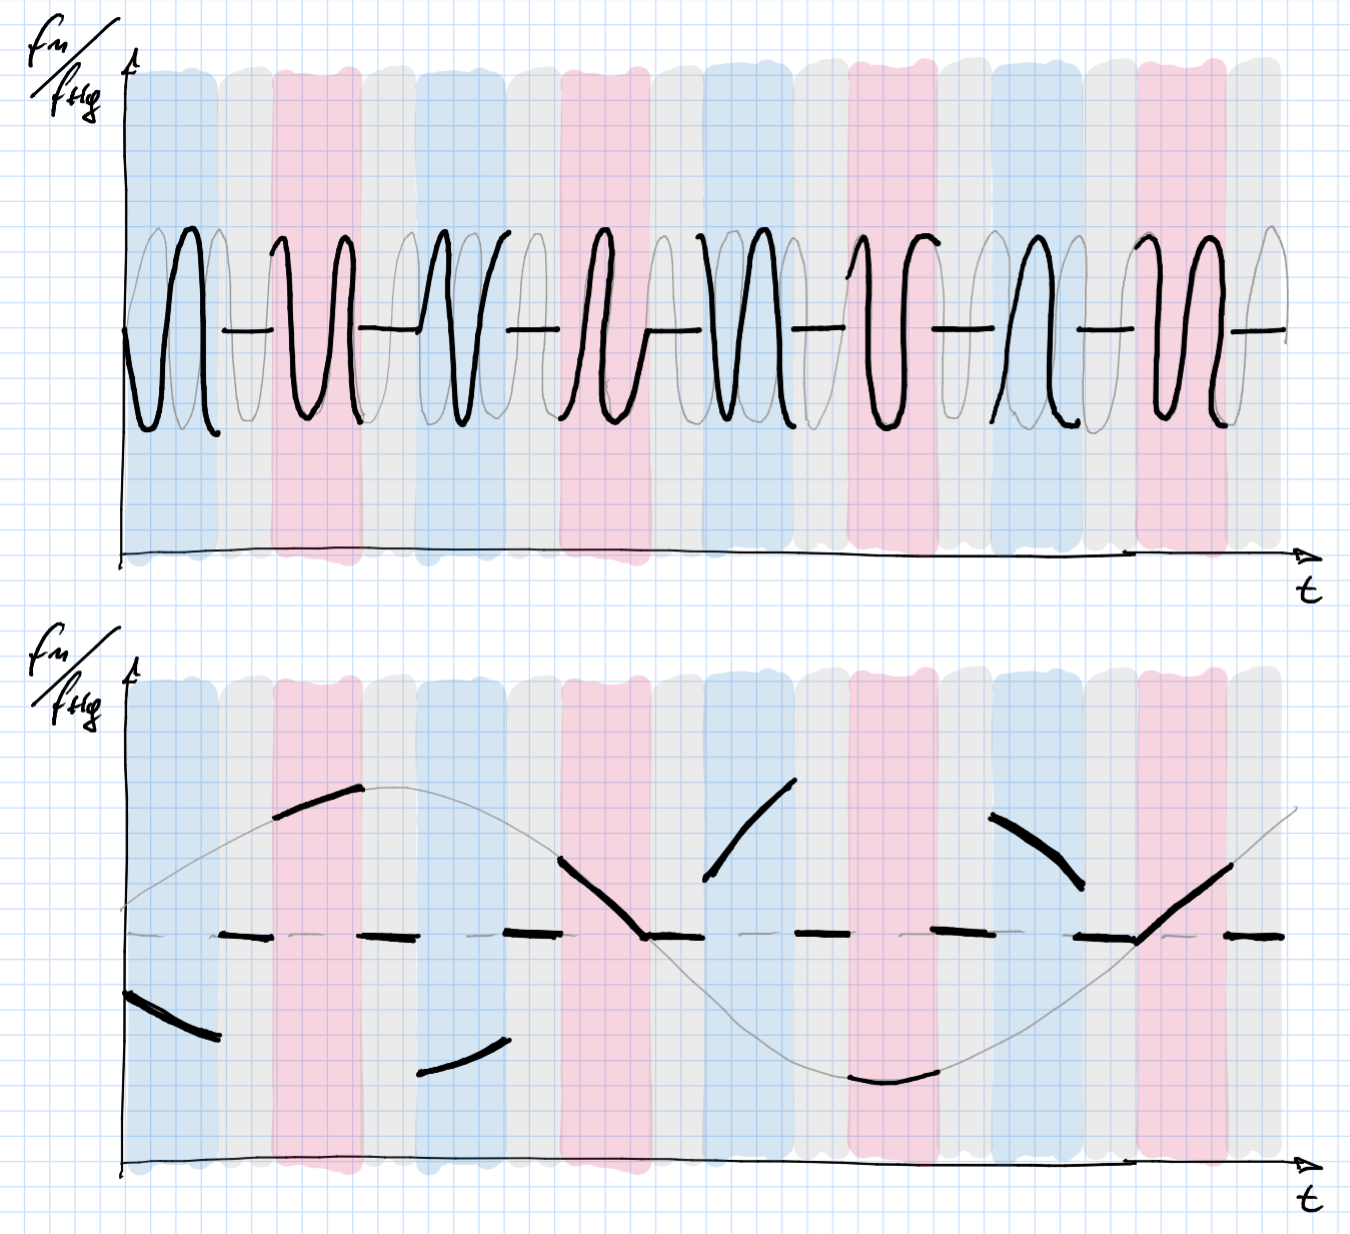
\includegraphics[width=.34\linewidth]{gfx/axions/data_taking_run}}
  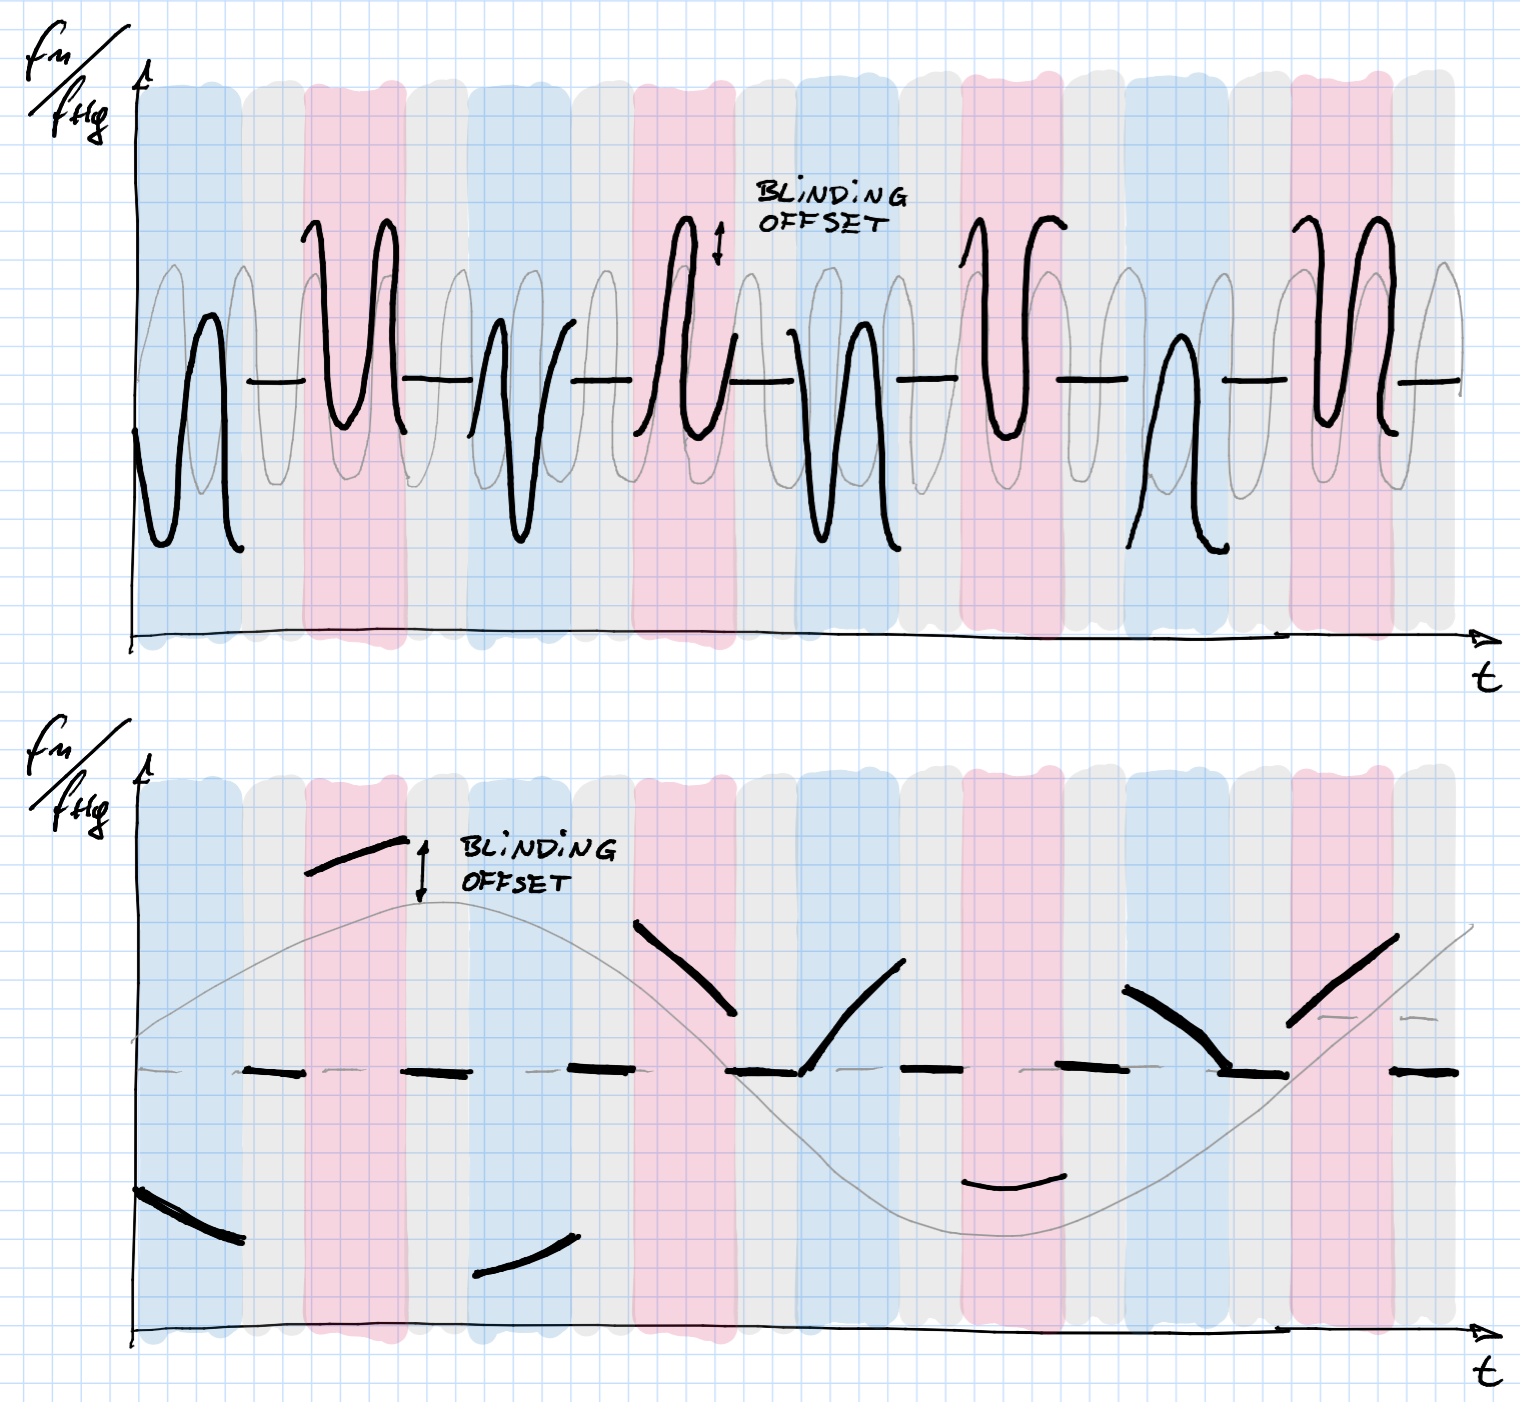
\includegraphics[width=.34\linewidth]{gfx/axions/data_taking_run_with_blinding}}
  \quad
  \subfloat
  [An oscillating neutron electric dipole moment signal in the nEDM @ PSI apparatus across many runs. The colours indicate different electric field states: parallel to the magnetic field, antiparallel to it and zero. Different runs have different magnetic field gradients, which causes each run to have a different shift in $R = f_n / f_{Hg}$.]
  {\label{fig:axions_data_taking_runs}
  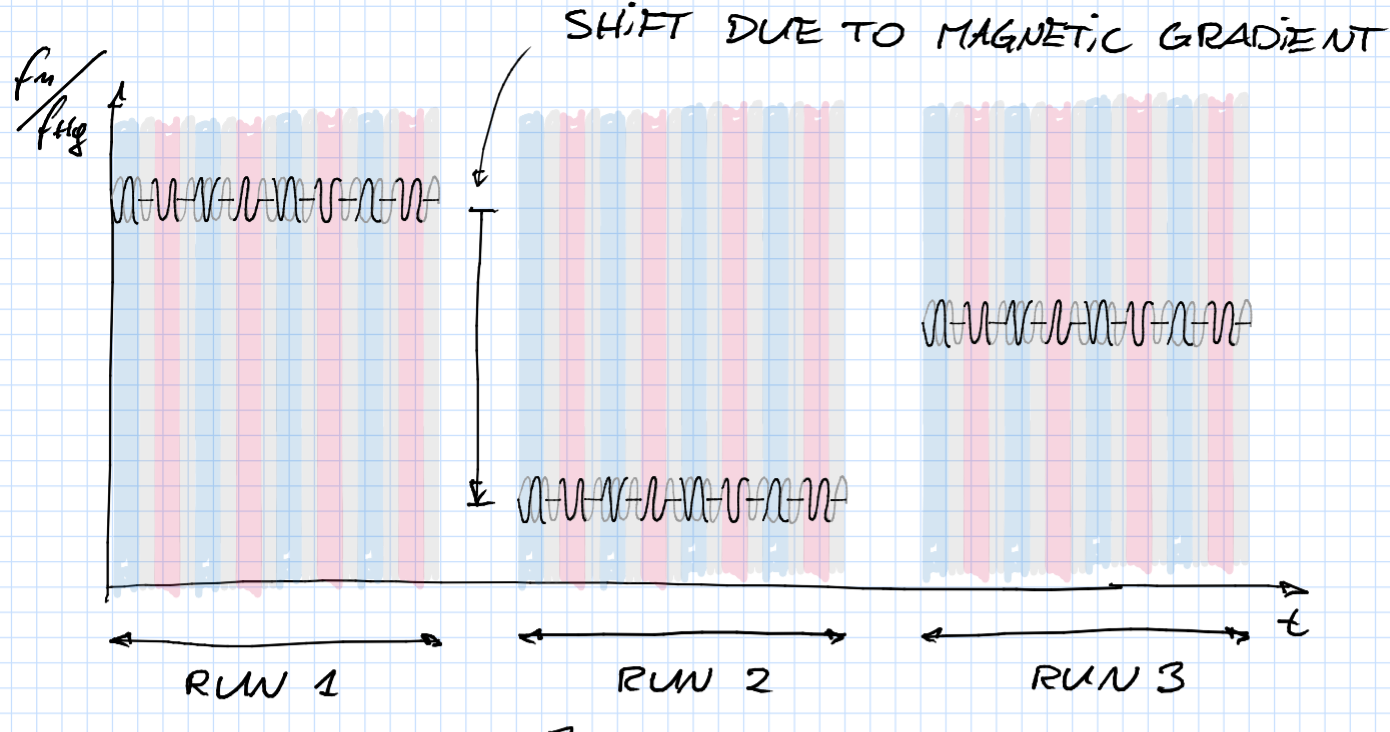
\includegraphics[width=.56\linewidth]{gfx/axions/data_taking_runs}}
  \caption{The data taking scheme in the nEDM experiment at PSI.}
\end{figure}

The vertical magnetic filed vertical gradient changes when a new \emph{run} is started. Thereby $R$ is shifted by a big value, changing the DC level of the oscillating nEDM signal, which is illustrated in Fig.\,\ref{fig:axions_data_taking_runs}. Moreover, even during a single \emph{run} the gradient drifts, as clearly visible in Fig.\,\ref{fig:axions_gradient_drift}.

The nEDM team spares no effort to measure the gradient. Nevertheless, the achieved precision ($\approx \unit[1]{pT/cm}$ is only comparable to the one of $f_n$ (in the order of \unit[1]{pT}). The exact way how the gradient should determined is highly non--trivial and there is ongoing research in this respect. Actually, even the height difference between the neturons and $^{199}$Hg centres of mass (a few milimeters) is still discussed. % Assuming a constant gradient during a \emph{run} one can determine it much more precise. This assumption, however, is known not to be exactly true.

\begin{figure}[bth]
  \myfloatalign
  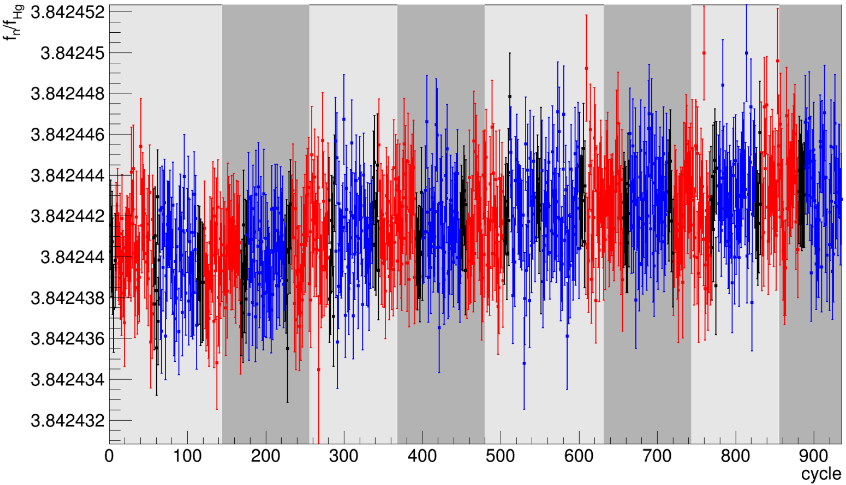
\includegraphics[width=.8\linewidth]{gfx/axions/gradient_drift_yoann}
  \caption
  [Drift of $R$]
  {%FIXME directly copied from Yoann's presentation on the 2015 PSI collaboration meeting
A typical time series of $R$ in the nEDM experiment. The colours depict electric field states, black being no electric field. A drift is clearly visible.}
  \label{fig:axions_gradient_drift}
\end{figure}

One should note, that any, including an oscillating one, nEDM effect affects only the position of the neutrons' resonance. The shape of the resonance curve is unaffected. Therefore, the method to extract neutron Larmor frequency $f_n$, and thereby $R$, for each \emph{cycle} is valid also in case of an oscillating nEDM.


\subsection{$R$ time series demodulation}
The time series of $R$ is not eligible for a Fourier--type analysis. The series has to be first demodulated into a coherent signal. To accound for the electric field changes, data taken at one configuration need to be \emph{flipped} around the DC level. Unfortunately, determining the DC level is not trivial.

Taking a look at Fig.\,\ref{fig:axions_gradient_drift} it becomes clear, that the $R$ value drifts. The main reason is a drift of the vertical gradient of the magnetic field. This effect could corrected for using the gradient measurement, as shown in Fig.\,\ref{fig:axions_gradient_drift_correction}. It is not straightforward, though, as there is not yet an established method to determine the gradient. The points taken at zero electric field provide additional information about the DC level. This, however, would have to be interpolated. The gradient drift correction is likely to turn out to be the most delicate part of the analysis.

\begin{figure}[bth]
  %FIXME directly copied from Elise's presentation on the 2015 PSI collaboration meeting
  \myfloatalign
  \subfloat
  [Another time series of $R$ in the nEDM experiment. The colours depict electric field states, black being no electric field. A drift is clearly visible.]
  {\label{fig:axions_gradient_drift_not_corrected}
  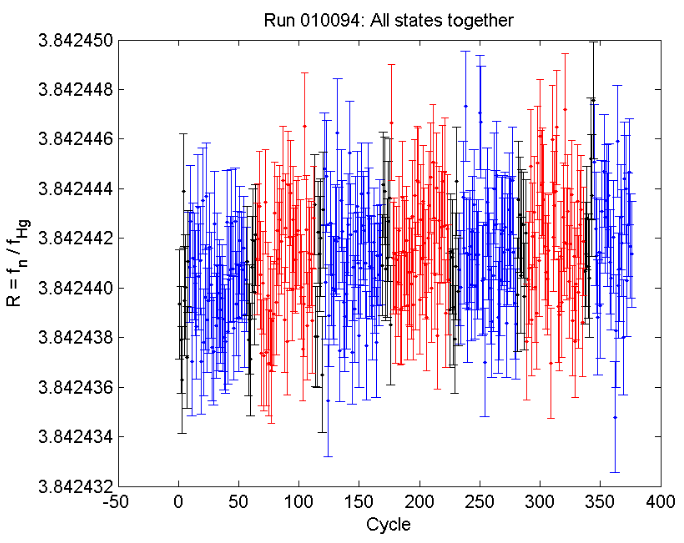
\includegraphics[width=.45\linewidth]{gfx/axions/gradient_drift_elise}}
  \quad
  \subfloat
  [The data as on Fig.\,\ref{fig:axions_gradient_drift_not_corrected} corrected for gradient fluctuations.]
  {\label{fig:axions_gradient_drift_corrected}
  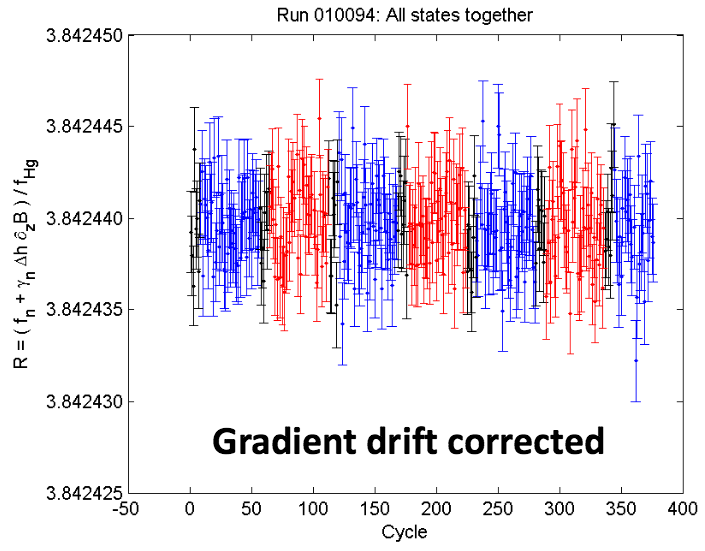
\includegraphics[width=.45\linewidth]{gfx/axions/gradient_drift_elise_corrected}}
  \caption{Correcting the $R$ time series for fluctuations of the vertical magnetic field gradient.}
  \label{fig:axions_gradient_drift_correction}
\end{figure}

% The gradient drift correction is likely to turn out to be the most delicate part of the analysis. One could consider two methods of tackling the problem. Firstly, the electric field configurations could be separated and analysed separately. In this case no correction for the gradient drift is necessary, although it
%
% Because of drift - not trivial to correct.
% Two analyses:
% 1. + and - HV separately -- the highest freqency is twice slower, but no correction necessary, but still possible. Gradient drift mimics a signal though.
% 2. try to correct for gradient and combine the data into one array








\section{The analysis itself}

\section{Axion-Wind analysis}

\section{Comparison of the analyses}
